% !TEX root=../pldi2019.tex



\section{Language}
\label{sec:language}


\subsection{Expressions}

\label{sub:expressions}
We take our host language to be a simply typed $\lambda$-calculus
extended with some basic types and \ML-style references.
The grammar in \autoref{fig:language-grammar} defines our language expressions.
Next to abstraction, application and variables,
we add constants for booleans, integers and strings.
We represent binary operations on these types by a $\star$.

The used extensions are \fixme{indicated} by the way we model tasks.
For the result of parallel tasks,
we need pairs.
An $\If{}{}{}$ expression comes in hand when defining guards.
To implement shared editors,
we will make use of references.
Creating a reference using the keyword $\Ref$ will result in a location $l$.
Locations are internal to the language and not intended to be directly manipulated by the programmer.
Dereferencing is done by using a bang,
for assigned one can use the $:=$ operator.
The unit value will be used as the result of an assignment.

\begin{figure}[h]
  \small
  \usemacro{G-Language-Compact}
  \caption{Language grammar} \label{fig:language-grammar}
\end{figure}

\label{sub:notation}
We will use double quotation marks ($\str{}$) to denote strings.
Integers are denoted by their decimal representation,
and booleans are written $\True$ and $\False$.
We will freely make use of the logic operators $\Not$, $\land$, and $\lor$,
arithmetic operators $+$, $-$, $\times$,
and the string append operator $\pp$.
Also, we will use the standard comparison operations $<$, $\le$, $\equiv$, $\not\equiv$, $\ge$, and $>$
as builtins.
Only when referring to operators in general we will use $\star$,
like in evaluation rules.
\label{sub:abbreviations}
Also, we will use the notation $e_1; e_2$
as an abbreviation for $(\lambda x:\Unit.\ e_2)\ e_1$,
and the notation $\Let x:\tau = e_1 \In e_2$
as an abbreviation for $(\lambda x:\tau.\ e_2)\ e_1$.
In both expressions $x$ is a fresh variable.

We will embed our task language into this basic language.
This means we can use all the power of the host language,
such as arithmetic operations and (higher order) functions,
in our task language.

\label{sub:pretasks}
The syntactic category $p$ of \emph{pretasks},
is further specified in \autoref{fig:task-grammar}.
A pretask $p$ is a task \emph{in making},
just as an expression is a value in making.
In the next subsections we will discuss each category of pretasks:
editors, steps and combinations.
As a general rule of thumb,
we will use open symbols ($\Edit, \Enter, \Next, \Xor$) where user input is required,
and closed symbols ($\Update, \Then, \Or$) where language constructs themself can make decisions.

\begin{figure}[h]
  \small
  \usemacro{G-Pretasks-Compact}
  \caption{Task grammar} \label{fig:task-grammar}
\end{figure}



\paragraph{Typing}

% Typing of our expressions $e$ is as to be expected.
% and won't be given in this document.
\Autoref{fig:type-grammar} shows the grammar of types used by \TOPHAT.
It contains standard types like functions, pairs, and unit,
some basic types, and a type for references.
The one difference with respect to standard work,
is the addition of a type for tasks: $\Task \tau$.

\begin{figure}[h]
  \small
  \usemacro{G-Types-Compact}
  \caption{Type grammar} \label{fig:type-grammar}
\end{figure}

Typing rules are of the form $\RelationT$,
which we read as \enquote{in environment $\Gamma$ and store typings $\Sigma$, expression $e$ has type $\tau$}.
The rules typing pretasks are given in \autoref{fig:typing-rules}.
The remaining constructs of our host language are standard,
therefore the typing rules for this part of our language are presented in the appendix.

\begin{figure}[h]
  \small
  \begin{mathpar}
    \boxed{\RelationT} \\
    \userule{T-Edit} \quad
    \userule{T-Enter} \quad
    \userule{T-Update} \\
    \userule{T-Then} \quad
    \userule{T-Next} \\
    \userule{T-And} \\
    \userule{T-Or} \quad
    \userule{T-Xor}\\
    \userule{T-Appoint} \quad
    \userule{T-Fail}
  \end{mathpar}
  \caption{Typing rules} \label{fig:typing-rules}
\end{figure}



\subsection{Editors}

In the introduction we claimed to create a language to model \emph{interactive} workflows.
By interaction we mean \emph{communication with people using the developed system}.
These end users should be able to enter information into the system,
change it, clear it, reenter it, etc.
To do this, we introduce the concept of an \emph{editor}.

Editors may or may not contain a current value.
When an editor has a value, it can be \emph{changed} or it can be \emph{emptied}.
When it is empty, a value can be \emph{filled}.
This is depicted as a state diagram in \autoref{fig:editor-state} below.

\begin{figure}[h]
  \centering
  \includegraphics[width=\columnwidth,page=3]{figures/drawings-crop.pdf}
  \caption{
    Possible states of an editor and its transitions.
    Note that shared editors cannot be cleared.
  }
  \label{fig:editor-state}
\end{figure}

One can consider editors as an abstraction over widgets in a \GUI,
form fields on a webpage,
or even sensors plugged into the system.
Take for example the input entry for age,
from \autoref{exm:flight-booking}.
Users can enter an integer, change it, remove it, enter another integer, and so on.
With editors we try to capture this \emph{constantly changing nature of user input}.
Also, because editors are \emph{typed},
they are only allowed to contain information of the right format,
as we have seen in \autoref{fig:flight-booking}.

How exactly information is entered is not of great importance.
This could be an input field for a string,
a switch for a boolean,
a spin box for an angle,
or even a map with a pin for a location.
% \Autoref{fig:editor-examples} depicts these examples.
\todo{Add figure with widget examples or not?}
In it's most banal form,
an editor is a line of text entered at a terminal and parsed to match
a string, boolean, angle or location value.



\paragraph{Valued and unvalued editors $(\Edit e, \Enter \tau)$}

At the core,
an editor is a container holding a value
or holding nothing.
Valued editors contain an expression $e$.
Therefore they inherit the type of $e$,
but embedded in the container type $\Task$.
This is expressed by the typing rule for valued editors \refrule{T-Edit}.

Unvalued editors do not have a value,
and therefore do not wrap an expression.
Because we strive to a fully typed system,
we have two options to type unvalued editors:
\begin{enumerate*}
  \item let the unvalued editor have a polymorphic type;
  \item annotate unvalued editors with a type and use that. \label{itm:annotate}
\end{enumerate*}

The first option sounds appealing.
However, consider the following use case.
We start with an editor containing the value two: $\Edit 2$.
The user can change this value, as long as it is an integer,
for example to five: $\Edit 5$.
Clearing the value results in an unvalued editor: $\Enter$.
Now, are we allowed to enter a value of some other type?
That is, can we now enter a string?
This would change the type of the editor
and violate the preservation theorem proved in \autoref{sub:preservation}!
Therefore,
we need to keep track of the type of values that can be entered into an unvalued editor
and we choose option (\ref{itm:annotate}).
The typing rule for valued editors can be found in \refrule{T-Enter}.

% Some examples of editors expressible in our language:
% \begin{itemize}
%   \item $\Edit 2$ is a valued editor which contains the integer value $2$.
%   \item $\Enter \String$ is an unvalued editor,
%     waiting for users to enter some string.
%   \item $\Edit ((\lambda x . x)\ 5)$ is a valued editor which,
%     after evaluation, will contain the value $5$.
%     (We will discuss evaluation of editors in the next section.)
% \end{itemize}


\paragraph{Shared editors $(\Update e)$}

Shared editors are a generalisation of normal editors discussed above.
Instead of \fixme{keeping} a value locally,
they watch a reference location.
Typing rule \refrule{T-Update} therefore states that,
for $\Update e$ to be a $\Task \tau$,
$e$ should be of type $\Reference \tau$.
Because \ML-style references always have a value,
shared editors cannot be cleared.
The value of the reference,
and thus the value of the stored editor,
can only be changed.
This is depicted in the second state diagram in \autoref{fig:editor-state}.

The consequence is that two completely different users can watch the same shared value
and get notified by changes the other makes.
Lets say Marco and Christopher both watch a shared editor of a coordinate.
We can visualise editors of this type by an input entry,
like we did in \autoref{exm:flight-booking},
but we could also choose to show a map with a pin.
When Marco moves this pin,
he will update the value of the shared editor,
and thus the value of the reference containing the coordinate.
This will be immediately reflected on Christopher's screen:
the pin will change its position on the map.
This way, Marco and Christopher can work together editing the same information.

\label{sub:time}
Another important use case for shared editors is sensors.
Sensors can be modelled by users updating the value of a shred editor once in a while.
Take for example the task to view the current time: \TS{update time}
which is a shared editor of type \TS{Task Int}.
% which is stored as a value of type $\Reference \Int$.
Every second, a clock sends a change event to the system.
Each shared editor watching the same location will be updated accordingly.
The value of a sensor is thus exposed through a shared editor.



\subsection{Steps}


% In the previous section we have set up our interaction model of inputs and actions,
% we defined our interactive component, the editor,
% and introduced the infinitely failing task.
Now that we have the core part of an interactive workflow,
namely editors,
we can continue with ways to compose multiple tasks.
Combining tasks can be done in two ways:
\begin{enumerate*}
  \item sequential or
  \item parallel.
\end{enumerate*}
For parallel composition we distinguish two kinds:
\begin{enumerate*}[(a)]
  \item pairing two tasks (\emph{and}-parallel); and
  \item choosing between two tasks (\emph{or}-parallel).
\end{enumerate*}
In this subsection we start with sequential composition.
The next subsection is about pairing and choosing.



\paragraph{Internal and external step $(e_1 \Then e_2, e_1 \Next e_2)$}

One might think that the best way to sequence tasks is by just following one task with another:
do this, then do that, then that, etc.
However, we like the continuation to depend on the value produced by the preceding task.
This way, we can use this information to precisely specify how to continue with work.
This is done by a \emph{step}.
We define a step from one task to another as
\begin{quote}
  a calculation which returns the next task to proceed with.
\end{quote}

To accomplish this,
we take continuations to be \emph{functions}.
These are just normal functions from our host language which,
when evaluated, result in something of type $\Task$.

The accompanied typing rules are \refrule{T-Then} and \refrule{T-Next}.
Note that typing ensures us that the left hand side $e_1$ will be a task delivering a value of type $\tau_1$.
The right hand side $e_2$ then, will use this value of type $\tau_1$,
and calculate a new task of type $\Task \tau_2$,
holding a value of (possibly another) type $\tau_2$.

There are two ways the decision can be made to step from one task to another:
% by the system or by the user.
internal or external.
% We call steps made by the system \emph{internal steps} ($\Then$).
% and \emph{external step} ($\Next$).
Internal steps are made by the system.
That is, the system decides when to proceed with the next task by rules specified by the programmer.
External steps are performed upon user's request.
Only when users decide to continue with the next task,
a step is taken.
Both internal and external steps can be guarded by using an $\If{}{}{}$ expression,
\todo{Change guarded to conditional}
as we will see in the next example.



\begin{example}[Conditional stepping]
\label{exm:conditions}

Take this little task.
\begin{TASK}
  enter Int >>= \n. if n == 42 then edit "Correct" else edit "Bad"
\end{TASK}
It asks users to enter an integer.
Only when the integer equals $42$, the next task will be a valued editor containing the string "Correct".
Otherwise, it will be an editor containing the string "Bad".

\end{example}




\paragraph{Fail $(\Fail)$}

The fail task has a special role in our language and semantics.
Conceptually, it is a task that \emph{never has a value} and \emph{never accepts user input}.
Like all other tasks, it also \emph{never ends}.
Because $\Fail$ will not produce a result,
it does not matter in which context we use this expression.
Therefore \refrule{T-Fail} states that it has type $\Task \tau$ for any type $\tau$.

The usage of $\Fail$ is to signal the failure to produce a sensible task to proceed with,
and, therefore, we have to continue with the current task.
One could think of it as the error value \CL{Nothing} from Haskell's \CL{Maybe} data type,
or \CL{None} from \ML's \CL{option}.
Note the difference between $\Fail$, $\Enter \tau$, and $\Edit \unit$.
The first is the failing task, which does not accept any input.
The second is an unvalued editor,
waiting for users to enter some information of type $\tau$ into the system.
The third is a valued editor containing the unit value.
This value can be cleared or reentered by users.
Both editors clearly have a future of user interaction,
the failing task does not.



\begin{example}[Failing guards]

Let us slightly change the guarded step from \autoref{exm:conditions}:
\begin{TASK}
  enter Int >>= \n. if n == 42 then edit "Correct" else fail
\end{TASK}
In place of of the task \TS{edit "Bad"} we use \TS{fail}.
This has the following consequence.
As long as the right hand side of $\Then$ does evaluate to $\Fail$,
users can indefinitely change the value of the editor to different integers,
possibly clearing it in between.
At the moment the value of the left hand side is $42$,
the right hand side will evaluate to the sensible task \TS{edit "Correct"},
and the step will be made.

\end{example}



\begin{example}[Wait]\label{exm:wait}

\lstset{emph={amount,start,now}}
Combining the language constructs we presented till now,
we can create a task that is idle for a requested amount of time.
To do this,
we make use of a shared editor holding the current time (see \autoref{sub:time}),
and a guarded internal step.
\begin{TASK}
  let wait : Int -> Task Unit = \amount : Int.
    update time >>= \start : Int.
    update time >>= \now : Int.
      if now >= start + amount then edit <<>> else fail
\end{TASK}
The first step is immediately taken.
It will result in \TS{start} to be the time at the moment \TS{wait} is executed.
Only when the current time \TS{now} is bigger or equal to the start time plus the asked delay,
the second step will be taken and we will continue with an editor holding the unit value.

\end{example}



\subsection{Side-by-side}



\paragraph{Parallel $(e_1 \And e_2)$}

\fixme{Write section on parallel}



\paragraph{Internal and external choice $(e_1 \Or e_2, e_1 \Xor e_2)$}

\fixme{Write section on choice}

\begin{example}[Delay]

\lstset{emph={n,proceed}}

To illustrate the usage of internal and external choices,
we will create an example which will ask users explicitly to proceed with a task or to cancel.
When users do not make a choice within a given amount of time,
we will automatically proceed.
To do this,
we will make user of the \TS{wait}-task from \autoref{exm:wait}.
\begin{TASK}
  let cancel : Task Unit = edit <<>> in
  let delay : Int -> Task Unit -> Task Unit =
    \n : Int. \proceed : Task Unit.
    (proceed <?> cancel) <|> (wait n >>= \u : Unit. proceed)
\end{TASK}
Note this task is higher-order:
it is a task which takes another task as a parameter.

\end{example}



\subsection{Annotations}

Lastly, pretasks can be annotated with additional information.
One could think of labelling information for buttons,
or description of tasks.
For now, we only concentrate on appointing tasks to users,
which is common in workflow modelling.



\paragraph{Appoint $(u \At e)$}

\fixme{Write section on users}
\begin{itemize*}
  \item How to create users?
  \item What is their type?
\end{itemize*}
